\documentclass[12pt]{article}

\usepackage[margin=2.5cm, a4paper]{geometry} % Rand
\usepackage{setspace} % Zeilenabstand

\usepackage[utf8]{inputenc}
\usepackage[ngerman]{babel}
\usepackage{pdfpages}
\usepackage{epigraph} 

\onehalfspacing % Zeilenabstand 1,5

\begin{document}

% \maketitle
% \thispagestyle{empty}
% \newpage

\begin{titlepage}
	\centering
	{\scshape\LARGE DHBW Karlsruhe\par}
	\vspace{1cm}
	{\scshape\Large Projekthandbuch\par}
	\vspace{1.5cm}
	{\huge\bfseries ClimateSight\par}
	\vspace{2cm}
	{\Large\itshape Leon Fertig (1142628)\\Matteo Kosina (2912404)\\Marius Kurth (3695338)\par}
	\vfill
	% \includegraphics[width=pagewidth]{Bilder/Titelbild.jpg}\par\vspace{1cm}
	\vfill

    % Bottom of the page
	{\large \today\par}
\end{titlepage}

\tableofcontents
\thispagestyle{empty}
\newpage

\setcounter{page}{1}


\section{Protokolle}
\begin{itemize}
	\item Inhalte sind u.a.:
	\begin{itemize}
		\item Zeitpunkt, Ort, Dauer, Teilnehmer
		\item Agenda
		\item wesentliche Inhalte (Kurzform)
		\item To-dos mit Zuständigkeiten, „erledigt bis“, Status, …
		\item Entscheidungen, …
	\end{itemize}
	\item Dokumentieren Sie Ihre Treffen und fügen die Protokolle dem Projekthandbuch in einem Kapitel
	zusammengefasst bei.
	\item Sie können auch die (weiter hinten geforderte) OPL für Protokollierung nutzen.
\end{itemize}

\section{Projektauftrag}
Projektauftrag konkretisieren ("Hinweis: Das Projekt sollte ein Team mit mehreren Leuten erfordern, einige Wochen oder
Monate dauern, Auftraggeber darf nicht identisch mit Projektleiter sein").
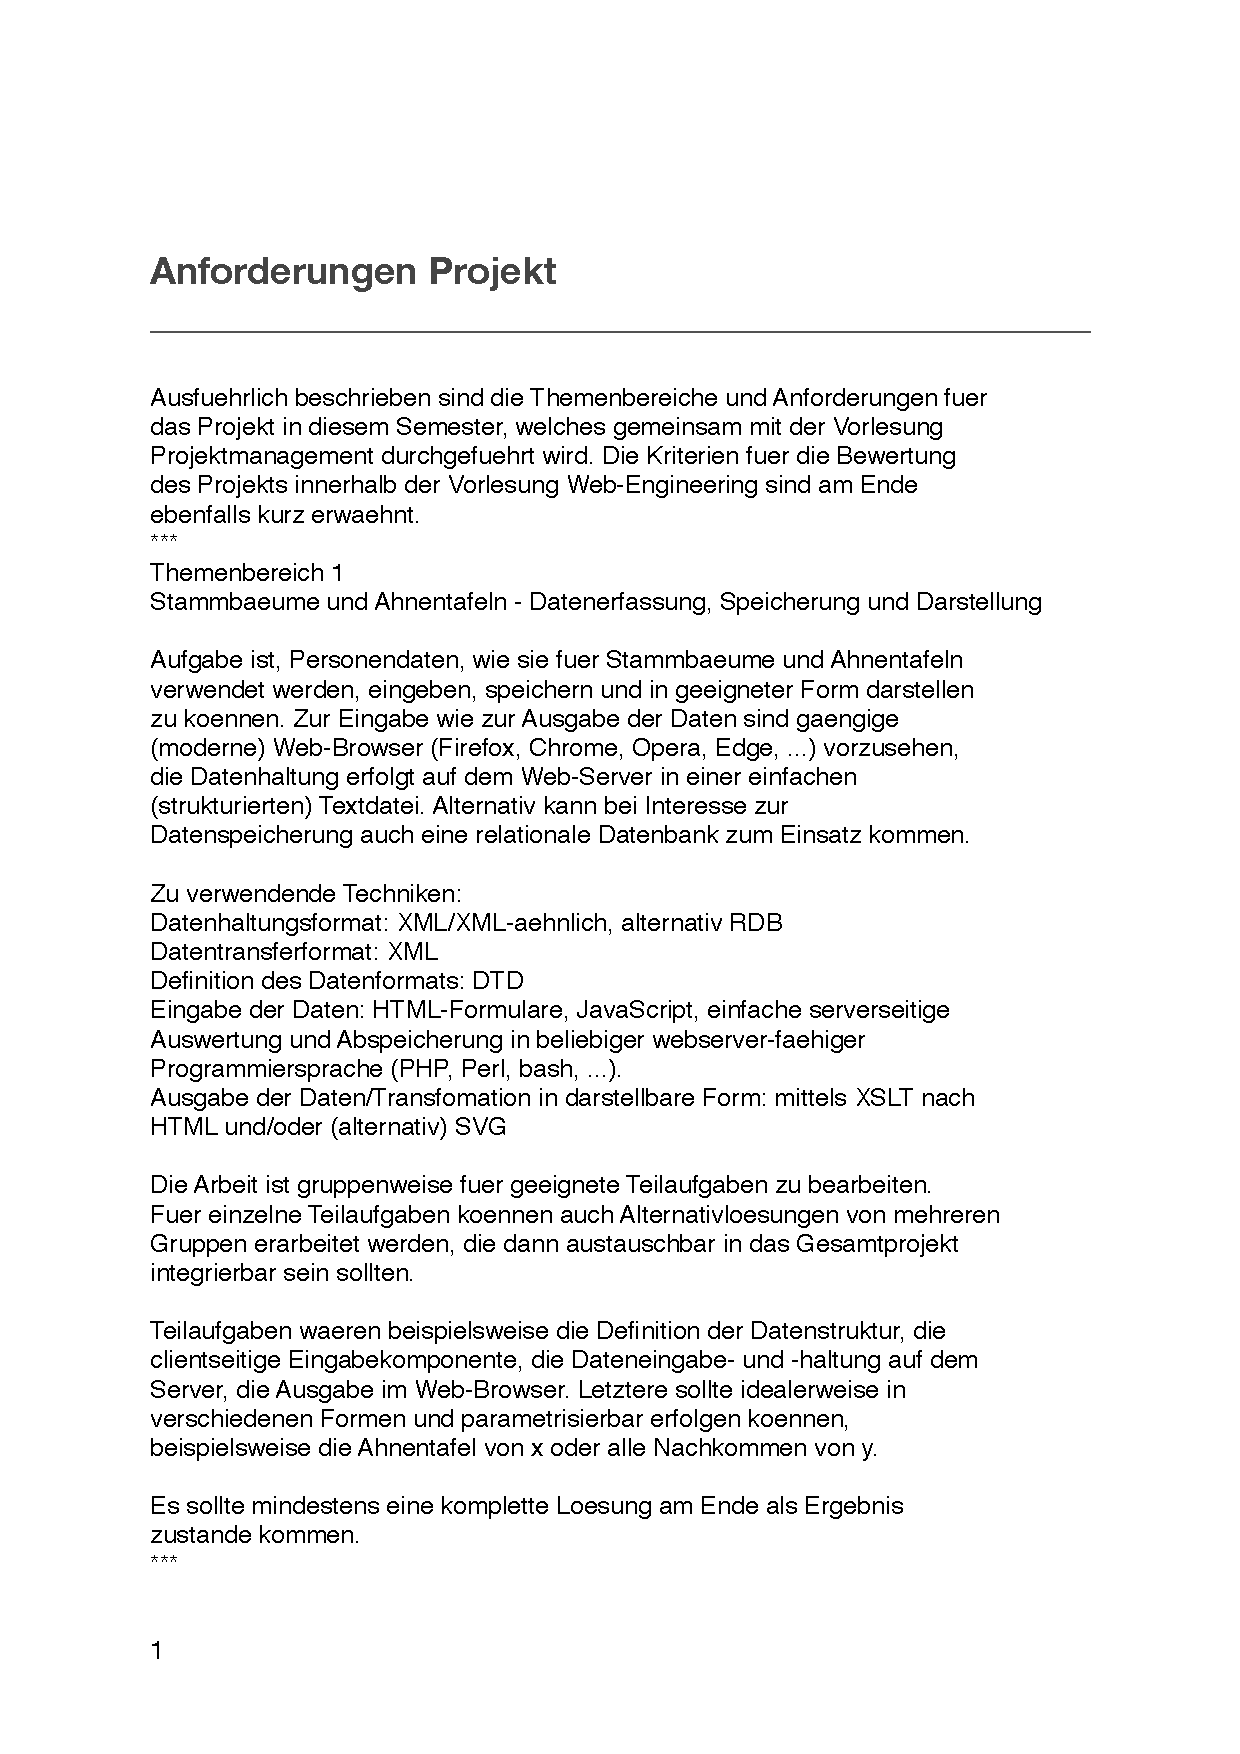
\includepdf[pages=-]{Planungsdokumente/Lastenheft.pdf}

\section{Projektziele}
Erstellen Sie die Projektziele für Ihr Projekt.
\begin{itemize}
\item Formulieren Sie die Ziele als vollständige Sätze aus. Bitte keine Stichworte!
\item Priorisieren Sie die Ziele nach der von Ihnen gewählten Methodik
\end{itemize}

\section{Projektplanung (Phasen- und Meilensteine)}

\section{Projektorganigramm}

\section{Offene-Punkte-Liste OPL}

\section{Projektstrukturplan PSP}
\begin{itemize}
	\item Erstellen Sie in Ihrem Team
	\item Projektstrukturplan (PSP)
	\item mindestens 6-8 Elemente
	\item Wenn möglich, sollten neben Arbeitspaketen auch Teilaufgaben oder Teilprojekte enthalten sein
	\item Erläutern Sie, welchen Gliederungstyp sie verwendet haben und erklären Sie am konkreten Fall warum
	\item Entwerfen Sie gemeinsam eine Vorlage für Arbeitspaketbeschreibungen
	\item Die Vorlage muss nicht als Bestandteil des Projekthandbuches hinzugefügt werden.
	\item Jedes Teammitglied erstellt mindestens eine Arbeitspaketbeschreibung
	\item Autor jedes Arbeitspaketes ist eindeutig kenntlich zu machen
\end{itemize}

\section{Arbeitspaketbeschreibungen}
s. PSP-Anforderungen

\section{Projektablaufplan, Gantt-Diagramm und Darstellung eines kritischen Pfades}
\begin{itemize}
	\item Auf Basis des PSP der vorherigen Aufgabe erstellen Sie
	\item Einen Ablaufplan
	\item Ein Gantt-Diagramm
	\item Welche Anordnungsbeziehungen enthält ihr Planung und erläutern Sie kurz warum
	\item Wo liegt der kritische Pfad?
	\item Gäbe es eine alternative Planung? Wenn ja, wie sähe die aus?
\end{itemize}

\section{Projektplanung (Ressourcen, Kosten, Risiko, Stakeholder)}
Auf Basis der Arbeitspakete eine Ressourcenplanung und eine Kostenplanung erstellen.\\
Analog: Kostengang und Kostensumme erarbeiten\\
Risikoanalyse
\begin{itemize}
	\item Zeigen auf, welche Arten von Risiken Sie identifiziert haben
	\item Wie ist ihre Risikomatrix ausgestaltet?
	\item Erläutern Sie anhand ausgesuchter Beispiele, warum Sie eine bestimmte Art der Risikobehandlung ausgewählt haben (z.B. Vermeidung oder Verlagerung)
\item Entscheiden Sie frei zwischen einer quantitativen und qualitativen Risikobewertung
\end{itemize}
Stakeholderanalyse
\begin{itemize}
	\item Erstellen Sie eine geeignete Vorlage, definieren Sie die Parameter
	\item Führen Sie beispielhaft einige Stakeholderanalyse durch
\end{itemize}



\section{Projektstatusbericht}
Statusbericht (etwa in der Hälfte des Projektzeitraumes)

\section{Product Backlog und Sprint Backlog}
Einen Product Backlog
\begin{itemize}
	\item Es sollten mindestens vier bis fünf User Stories enthalten sein
	\item Fügen Sie auch ein Epic Beispiel ein
\end{itemize}
Sprint Backlog

→ Es sollten mindestens vier bis fünf Tasks/Aufgaben enthalten sein


\end{document}
